\section{Quantenmechanik}

\subsection{Photoelektrischer Effekt}
	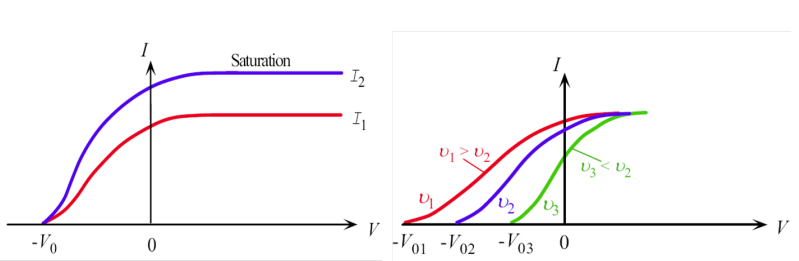
\includegraphics[width=0.99\columnwidth]{Bilder/Photoeffekt_2}

	\begin{minipage}{0.58\linewidth}
		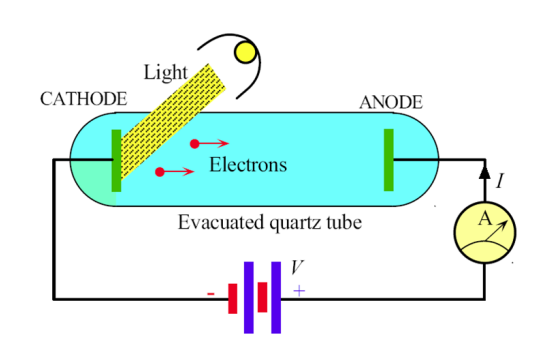
\includegraphics[width=0.99\linewidth]{Bilder/Photoeffekt_1}
	\end{minipage}
	\hfill
	\begin{minipage}{0.4\linewidth}
		\begin{itemize}
			\item I fotoni che colpiscono la piastra espellono gli elettroni.
			\item La corrente è determinata \textbf{solamente} dall'intensità della luce (nr. fotoni)
			\item $V_0$ ovvero l' $E_{kin}$ degli elettroni dipende \textbf{solo} dalla lunghezza d'onda della luce
		\end{itemize}
	\end{minipage}

	Die Bremsspannung hängt laut der Grafik \textbf{nur} von der Lichtfrequenz ab.

\subsubsection{Compton Effekt}\vspace{-1em}

\begin{minipage}{0.58\columnwidth}
	Ein Photon wird an einem Elektron gestreut und gibt dabei Energie an das Elektron ab. 
	Das gestreute Photon hat eine längere Wellenlänge als das einfallende Photon.
	
	Mit den Folgenden Gleichungen kann durch Impulserhaltung geschlussfolgert werden, 
	dass ein Photon sowohl ein Teilchen als auch eine Welle ist. Mit der Impulserhaltung folgt:	
\end{minipage}\hfill
\begin{minipage}{0.4\columnwidth}
	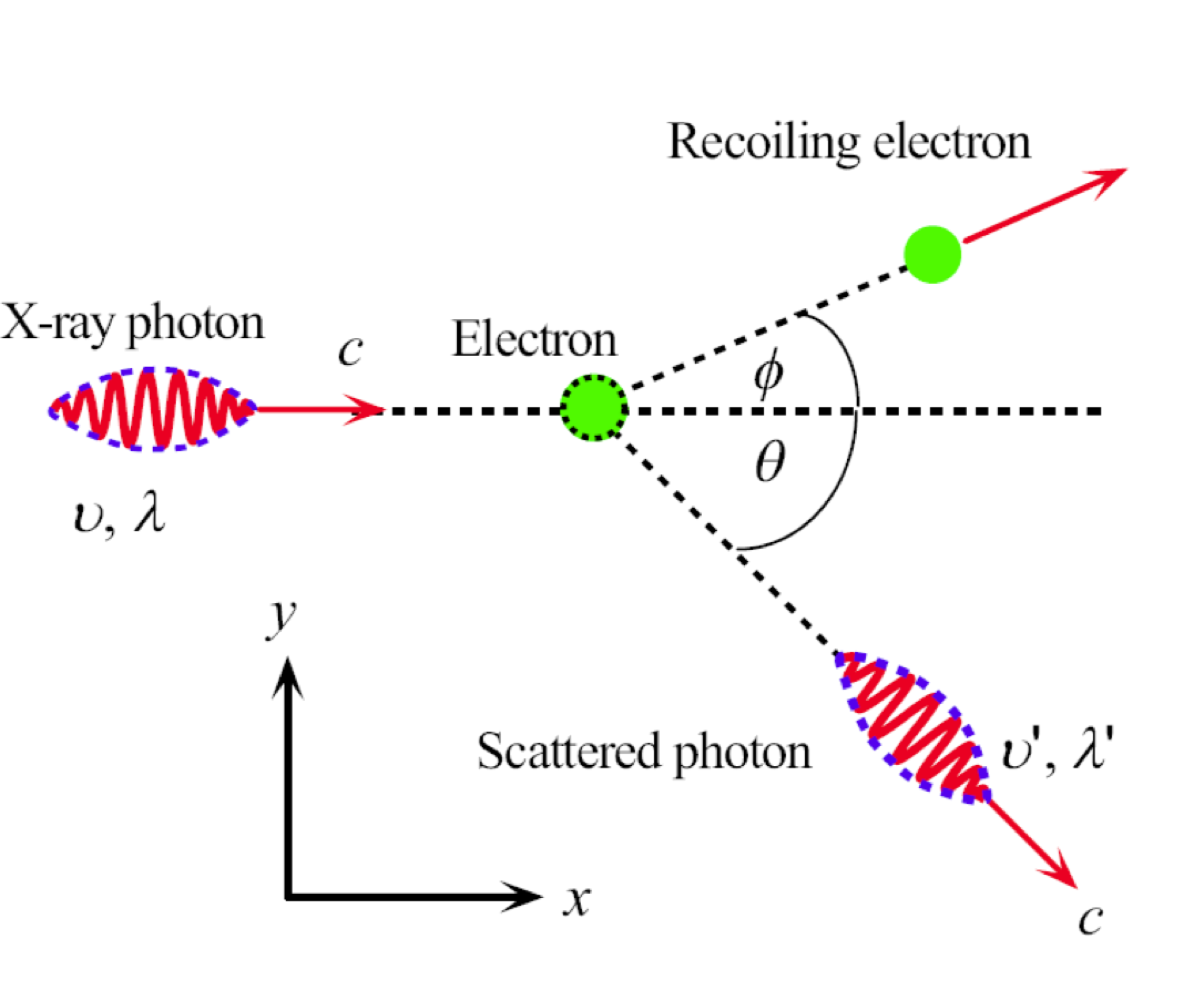
\includegraphics[width=\linewidth]{Bilder/copmton_effekt.png}
\end{minipage}

\renewcommand{\arraystretch}{1.9}
\begin{tabular}{lll}
    Energie des Elektrons & $\displaystyle E_{e} = \frac{1}{2} m v^{2}$ & \\ 
    Energie des Photons & $\displaystyle E_{\gamma} = h \cdot \frac{c}{\lambda}$ & \\ 
    Compton Effekt & $\displaystyle \Delta \lambda = \frac{h}{m_{e} \cdot c} (1 - \cos\theta)$ & \\ 
    Potenza interna & $\displaystyle P_{int} = \frac{P_{out}}{T}$ & $T = \text{trasmissività (in \%)}$ \\ 
    Energia cavità & $\displaystyle E_k = 2 \cdot P_{int} \cdot \frac{l}{c}$ & 2 Perchè fa avanti e indietro\\
\end{tabular}
\renewcommand{\arraystretch}{1}


\subsection{Die Schrödinger-Gleichung und der Tunneleffekt}
In der Quantenmechanik besitzen Teilchen nicht mehr einen festen Ort und einen klar definierten Impuls. 
Quantenmechanisch treten nur noch Aufenthaltswahrscheinlichkeiten auf. 
Diese wird durch die Wellenfunktion $\Psi \left(\stackrel{\to }{x},t\right)$ beschrieben. 
Wie diese Wellenfunktion aussieht, beschreibt die Schrödinger-Gleichung ("Bewegungsgleichung" der Quantenmechanik):

\begin{minipage}{0.5\linewidth}
	\[\frac{\diff^2\Psi (x)}{\diff x^2}+\frac{2m}{{\hbar }^{2}}\left(E-V\left(x\right)\right)\Psi \left(x\right)=0\]
\end{minipage}
% \hfill
\begin{minipage}{0.28\linewidth}
	\begin{align*}
		m &= \text{Masse}\\
		V(x) &= \text{Potential}\\
		E &= \text{Energie}
	\end{align*} 
\end{minipage}

Die Wellenfunktion beschreibt die ortsaufgelöste Aufenthaltswahrsch. eines Teilchens: 
\[
	|\Psi(\vec{x}, t)|^2 \diff x = \Psi(\vec{x}, t) \cdot \Psi^*(\vec{x}, t) 
\]

\subsubsection{Tunneleffekt}
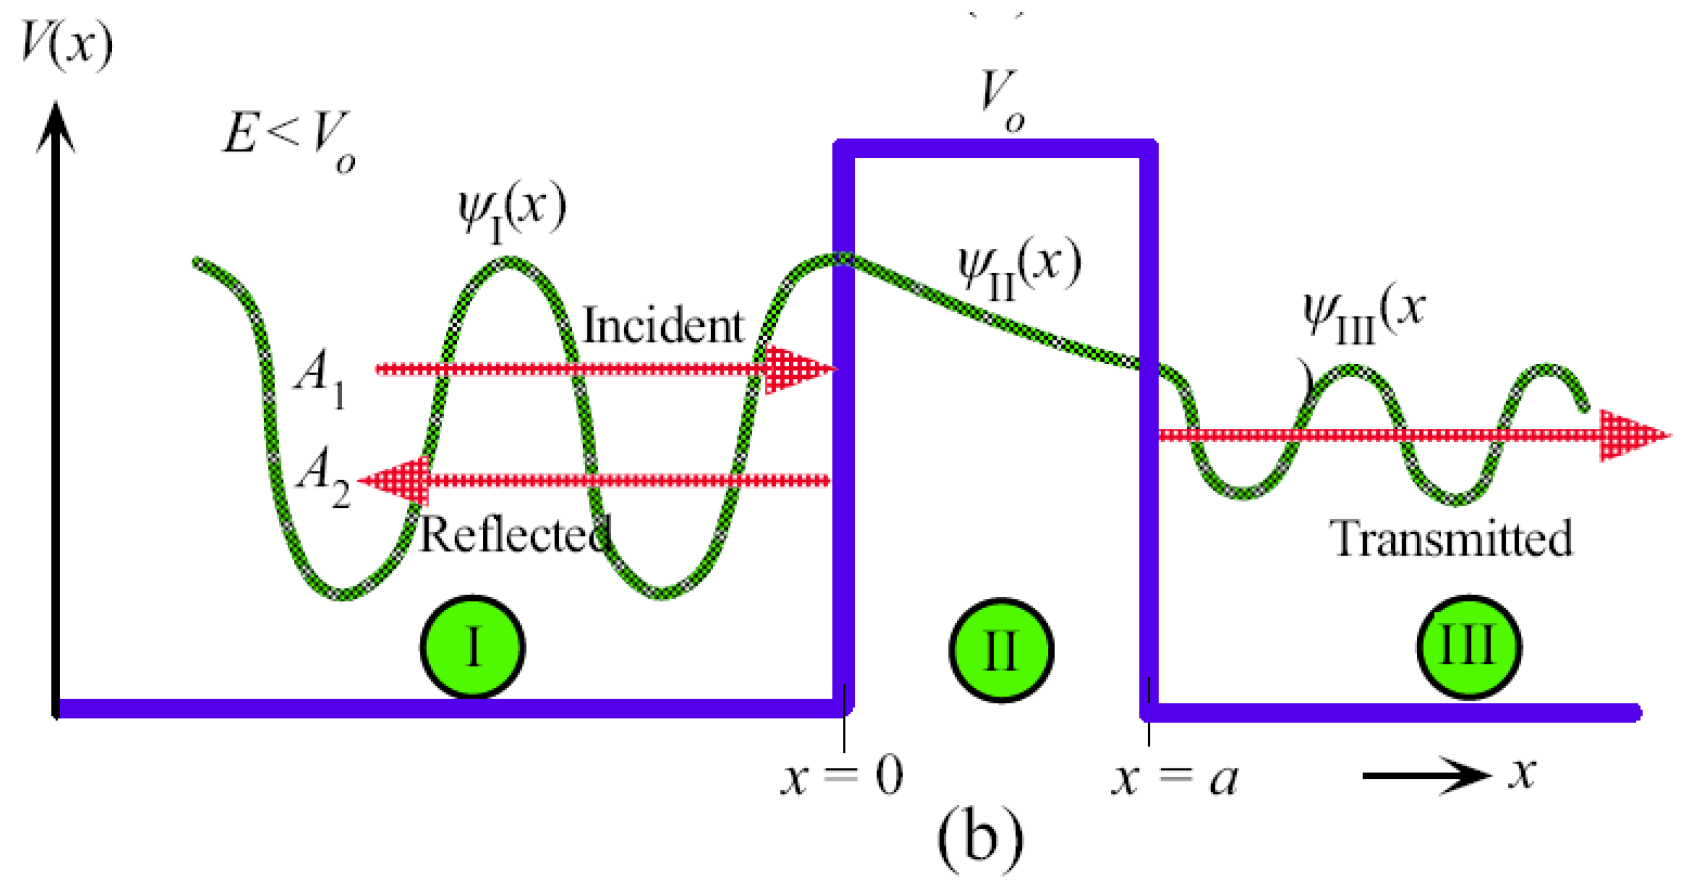
\includegraphics[width=0.99\linewidth]{Bilder/Tunneleffekt}
Wenn ein Teilchen auf eine Potentialbarriere trifft, gibt es quantenmechanisch eine \textbf{endliche Warscheinlichkeit}, 
dass das Teilchen durch diese hindurch tunnelt. Dies geschieht, auch wenn klassisch gesehen das Teilchen 
zu wenig Energie hat, die Barriere zu überwinden. Somit ist der Tunneleffekt \textit{rein quantenmechanisch} und 
auch nur so erklärbar.

Der Transmissions- ($T$) und Reflektionskoeffizient ($R$) hängt von der Höhe und Breite der Barriere ab. 
Je grösser sie wird, desto mehr nähert man sich der klassischen Physik, da kein Tunneleffekt mehr auftritt.

Der Tunneleffekt ist ein fundamentales Problem bei der Miniaturisierung von Halbleiterbauteilen

Eine Anwendung vom Tunneleffekt ist das Rastertunnel-Elektronenmikroskop(STM). 
Dabei kann man mit einer atomar-scharfen Spitze eine Oberfläche abrastern und 
dabei mit atomarer Auflösung die Oberfläche charakterisieren. $R+T = 1$!

$$ R = \dfrac{|B_Ie^{-ikx}|^2}{|A_Ie^{-ikx}|^2} = \frac{(\alpha^2 + k^2)^2 \sinh^2(\alpha a)}{(\alpha^2 + k^2)^2 \sinh^2(\alpha a) + 4k^2\alpha^2}$$
$$T = \dfrac{|A_{III}e^{-ikx}|^2}{|A_Ie^{-ikx}|^2} = \frac{4k^2\alpha^2}{(\alpha^2 + k^2)^2 \sinh^2(\alpha a) + 4k^2\alpha^2}  $$